\PassOptionsToPackage{unicode=true}{hyperref} % options for packages loaded elsewhere
\PassOptionsToPackage{hyphens}{url}
\documentclass[10pt,dvipsnames,ignorenonframetext,aspectratio=169]{beamer}
\IfFileExists{pgfpages.sty}{\usepackage{pgfpages}}{}
\setbeamertemplate{caption}[numbered]
\setbeamertemplate{caption label separator}{: }
\setbeamercolor{caption name}{fg=normal text.fg}
\beamertemplatenavigationsymbolsempty
\usepackage{lmodern}
\usepackage{amssymb,amsmath}
\usepackage{ifxetex,ifluatex}
\usepackage{fixltx2e} % provides \textsubscript
\ifnum 0\ifxetex 1\fi\ifluatex 1\fi=0 % if pdftex
  \usepackage[T1]{fontenc}
  \usepackage[utf8]{inputenc}
\else % if luatex or xelatex
  \ifxetex
    \usepackage{mathspec}
  \else
    \usepackage{fontspec}
\fi
\defaultfontfeatures{Ligatures=TeX,Scale=MatchLowercase}







\fi

  \usetheme[]{monash}

  \usecolortheme{monashwhite}


% A default size of 24 is set in beamerthememonash.sty

% Title page
\setbeamertemplate{title page}
{\placefig{-0.01}{-0.01}{width=1.01\paperwidth,height=1.01\paperheight}{daffodil\_seeds.jpg}
\begin{textblock}{7.5}(1,2.8)\usebeamerfont{title}
{\color{white}\raggedright\par\inserttitle}
\end{textblock}
\begin{textblock}{7.5}(1,7)
{\color{white}\raggedright{\insertauthor}\mbox{}\\[0.2cm]
\insertdate}
\end{textblock}}


  \useinnertheme{rounded}

  \useoutertheme{smoothtree}

% use upquote if available, for straight quotes in verbatim environments
\IfFileExists{upquote.sty}{\usepackage{upquote}}{}
% use microtype if available
\IfFileExists{microtype.sty}{%
  \usepackage{microtype}
  \UseMicrotypeSet[protrusion]{basicmath} % disable protrusion for tt fonts
}{}


\newif\ifbibliography


\hypersetup{
      pdftitle={Remote sensing: concepts and applications; Image processing and interpretation},
            colorlinks=true,
    linkcolor=red,
    citecolor=Blue,
    urlcolor=blue,
    breaklinks=true}
%\urlstyle{same}  % Use monospace font for urls







% Prevent slide breaks in the middle of a paragraph:
\widowpenalties 1 10000
\raggedbottom

  \AtBeginPart{
    \let\insertpartnumber\relax
    \let\partname\relax
    \frame{\partpage}
  }
  \AtBeginSection{
    \ifbibliography
    \else
      \let\insertsectionnumber\relax
      \let\sectionname\relax
      \frame{\sectionpage}
    \fi
  }
  \AtBeginSubsection{
    \let\insertsubsectionnumber\relax
    \let\subsectionname\relax
    \frame{\subsectionpage}
  }



\setlength{\parindent}{0pt}
\setlength{\parskip}{6pt plus 2pt minus 1pt}
\setlength{\emergencystretch}{3em}  % prevent overfull lines
\providecommand{\tightlist}{%
  \setlength{\itemsep}{0pt}\setlength{\parskip}{0pt}}

  \setcounter{secnumdepth}{0}


%% Monash overrides
\AtBeginSection[]{
   \frame<beamer>{
   \frametitle{Outline}\vspace*{0.2cm}
   
   \tableofcontents[currentsection,hideallsubsections]
  }}

% Redefine shaded environment if it exists (to ensure text is black)
\ifcsname Shaded\endcsname
  \definecolor{shadecolor}{RGB}{225,225,225}
  \renewenvironment{Shaded}{\color{black}\begin{snugshade}\color{black}}{\end{snugshade}}
\fi
%%

\newlength{\cslhangindent}
\setlength{\cslhangindent}{1.5em}
\newenvironment{CSLReferences}%
  {}%
  {\par}

  \usepackage{setspace}
  \usepackage{wasysym}
  % \usepackage{footnote} % don't use this this breaks all
  \usepackage{fontenc}
  \usepackage{fontawesome}
  \usepackage{booktabs,siunitx}
  \usepackage{longtable}
  \usepackage{array}
  \usepackage{multirow}
  \usepackage{wrapfig}
  \usepackage{float}
  \usepackage{colortbl}
  \usepackage{pdflscape}
  \usepackage{tabu}
  \usepackage{threeparttable}
  \usepackage{threeparttablex}
  \usepackage[normalem]{ulem}
  \usepackage{makecell}
  \usepackage{xcolor}
  \usepackage{tikz} % required for image opacity change
  \usepackage[absolute,overlay]{textpos} % for text formatting
  \usepackage{chemfig}
  \usepackage[skip=0.333\baselineskip]{caption}
  % \newcommand*{\AlignChar}[1]{\makebox[1ex][c]{\ensuremath{\scriptstyle#1}}}%

  % this font option is amenable for beamer
  \setbeamerfont{caption}{size=\tiny}
  \singlespacing
  \definecolor{lightgrayd}{gray}{0.95}
  \definecolor{skyblued}{rgb}{0.65, 0.6, 0.94}
  \definecolor{oranged}{RGB}{245, 145, 200}

  % \newlength{\cslhangindent}
  % \setlength{\cslhangindent}{1.5em}
  % \newenvironment{cslreferences}%
  %   {\setlength{\parindent}{0pt}%
  %   \everypar{\setlength{\hangindent}{\cslhangindent}}\ignorespaces}%
  %   {\par}


  \newcommand{\bcolumns}{\begin{columns}[T, onlytextwidth]}
  \newcommand{\ecolumns}{\end{columns}}

  \newcommand{\bdescription}{\begin{description}}
  \newcommand{\edescription}{\end{description}}

  \newcommand{\bitemize}{\begin{itemize}}
  \newcommand{\eitemize}{\end{itemize}}
  \AtBeginSubsection{}
  \captionsetup{skip=0pt,font=tiny,belowskip=0pt,aboveskip=0pt}

  \title[]{Remote sensing: concepts and applications; Image processing
and interpretation}


  \author[
        Deependra Dhakal\\
Assistant Professor\\
\textit{ddhakal.rookie@gmail.com}\\
\url{https://rookie.rbind.io}
    ]{Deependra Dhakal\\
Assistant Professor\\
\textit{ddhakal.rookie@gmail.com}\\
\url{https://rookie.rbind.io}}


\date[
      
  ]{
    }

\begin{document}

% Hide progress bar and footline on titlepage
  \begin{frame}[plain]
  \titlepage
  \end{frame}


   \frame<beamer>{
   \frametitle{Outline}\vspace*{0.2cm}
   
   \tableofcontents[hideallsubsections]
  }

\hypertarget{remote-sensing}{%
\section{Remote sensing}\label{remote-sensing}}

\begin{frame}{Background}
\protect\hypertarget{background}{}
\begin{columns}[T, onlytextwidth]
\column{0.6\textwidth}

\begin{itemize}
\item History may be traced back to the first pre-historic explorer who climbed a nearby hill to study the lay of the land.
\item During first half of 19th century, Louis Jacques Mande Daguerre and Joseph Nicephore Niepc invented a photographic device, a foundation for modern photography and a means to record a remotely sensed image.
\item In 1859, Gaspard Félix Tournachon Clateu (later known in the literature as Félix Nadar) took the first known aerial image from a balloon.
\end{itemize}
\column{0.4\textwidth}

\begin{figure}
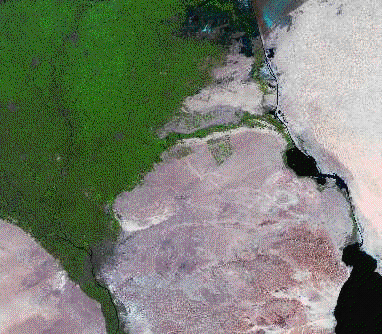
\includegraphics[width=0.88\linewidth]{../images/landsat_mss_september20_1984_nile_delta} \caption{Landsat MSS image acquired September 20, 1984 over the Nile Delta area.}\label{fig:historical-landsat}
\end{figure}

\end{columns}
\end{frame}

\begin{frame}{Meaning}
\protect\hypertarget{meaning}{}
\bcolumns
\column{0.65\textwidth}
\footnotesize

\begin{itemize}
\tightlist
\item
  Remote sensing provides data at a synoptic global level that is
  impossible to replicate with in situ measurements.
\item
  Remote sensing imagery used for the identification of earth surface
  features is dependent upon measurable variations in electromagnetic
  field strength. Variations are mainly three types:

  \begin{enumerate}
  \scriptsize
  \item Spectral
  \item Spatial
  \item Temporal
  \end{enumerate}
\item
  Simply, the measurement of an object by a device that is not in
  physical contact is \alert{remote sensing}.

  \begin{itemize}
  \scriptsize
  \item Active remote sensing involves transmission and reception of radiation, such as radar/lidar (CLOUDSAT/CALIPSO)
  \item Passive remote sensing only receives radiation from a target of interest, such as MODIS, Sentinel, Landsat and majority of earth orbiting sensor systems
  \end{itemize}
\end{itemize}

\column{0.35\textwidth}

\begin{figure}
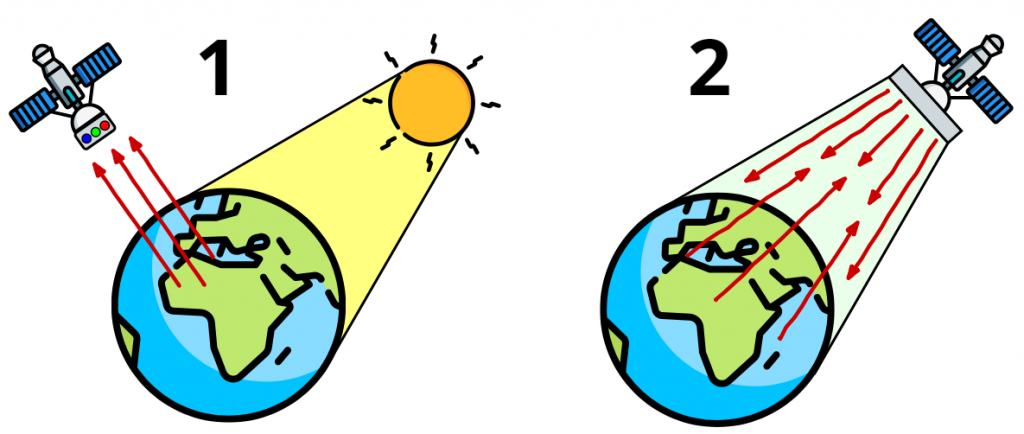
\includegraphics[width=0.95\linewidth]{../images/active_passive_remote_sensing} \caption{Passive (left) and active (right) remote sensing.}\label{fig:active-passive-remote}
\end{figure}

\ecolumns
\end{frame}

\begin{frame}{}
\protect\hypertarget{section}{}
\begin{itemize}
\tightlist
\item
  The principal source for the images is the electromagnetic (EM) energy
  spectrum.
\item
  The spectral bands are grouped according to energy per photon ranging
  form the gamma rays (highest energy) to the radio waves (lowest
  energy)
\end{itemize}

\begin{figure}
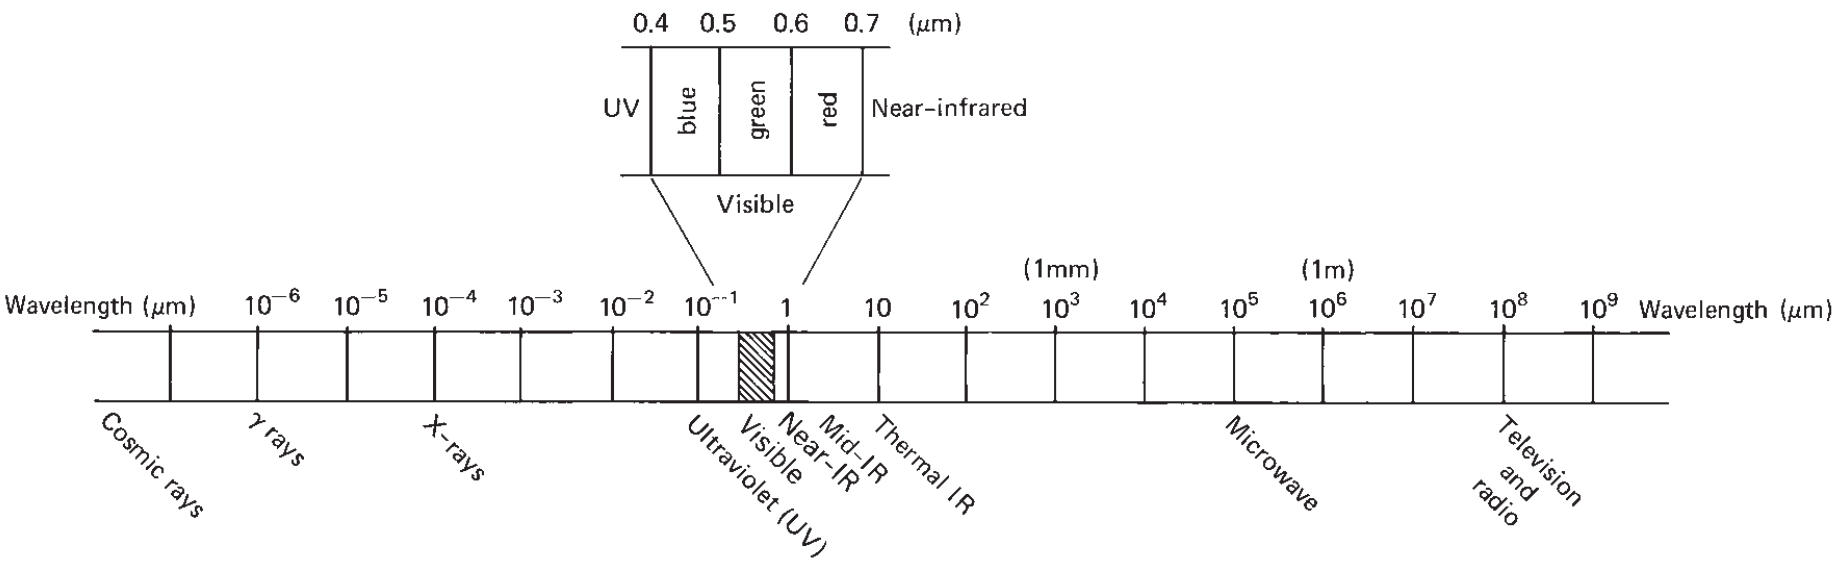
\includegraphics[width=0.85\linewidth]{../images/spectral_bands_electromagnetic_wavelength} \caption{Electromagnetic spectrum}\label{fig:electromagnetic-spectrum}
\end{figure}
\end{frame}

\begin{frame}{}
\protect\hypertarget{section-1}{}
\bcolumns
\column{0.33\textwidth}

\begin{figure}
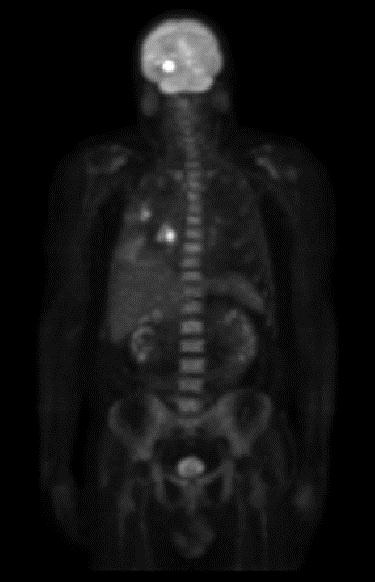
\includegraphics[width=0.7\linewidth]{../images/gamma-ray-imaging} \caption{$\gamma$-ray imaging is used in nuclear medicine and astronomical observations.}\label{fig:gamma-ray-imaging}
\end{figure}

\column{0.33\textwidth}

\begin{figure}
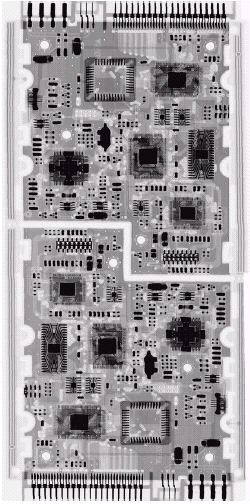
\includegraphics[width=0.6\linewidth]{../images/x-ray-imaing-industrial-process} \caption{x-ray imaging is widely used in medical imaging as well as industrial imaging (of circuit boards, for example).}\label{fig:x-ray-imaging}
\end{figure}

\column{0.33\textwidth}

\begin{figure}
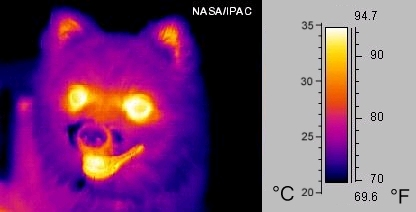
\includegraphics[width=0.75\linewidth]{../images/Infrared_dog} \caption{Infrared band imaging provides an indication of thermal profile of a scene.}\label{fig:infrared-imaging}
\end{figure}

\ecolumns

(\scriptsize Refer to Section 1.2 of Lillesand, Kiefer, and Chipman
(2015) for ``Energy sources and radiation principles'' and 1.3 and 1.4
for detailed exploration of theoretical basis of electromagnetic wave
information generation.)
\end{frame}

\begin{frame}{}
\protect\hypertarget{section-2}{}
\begin{figure}
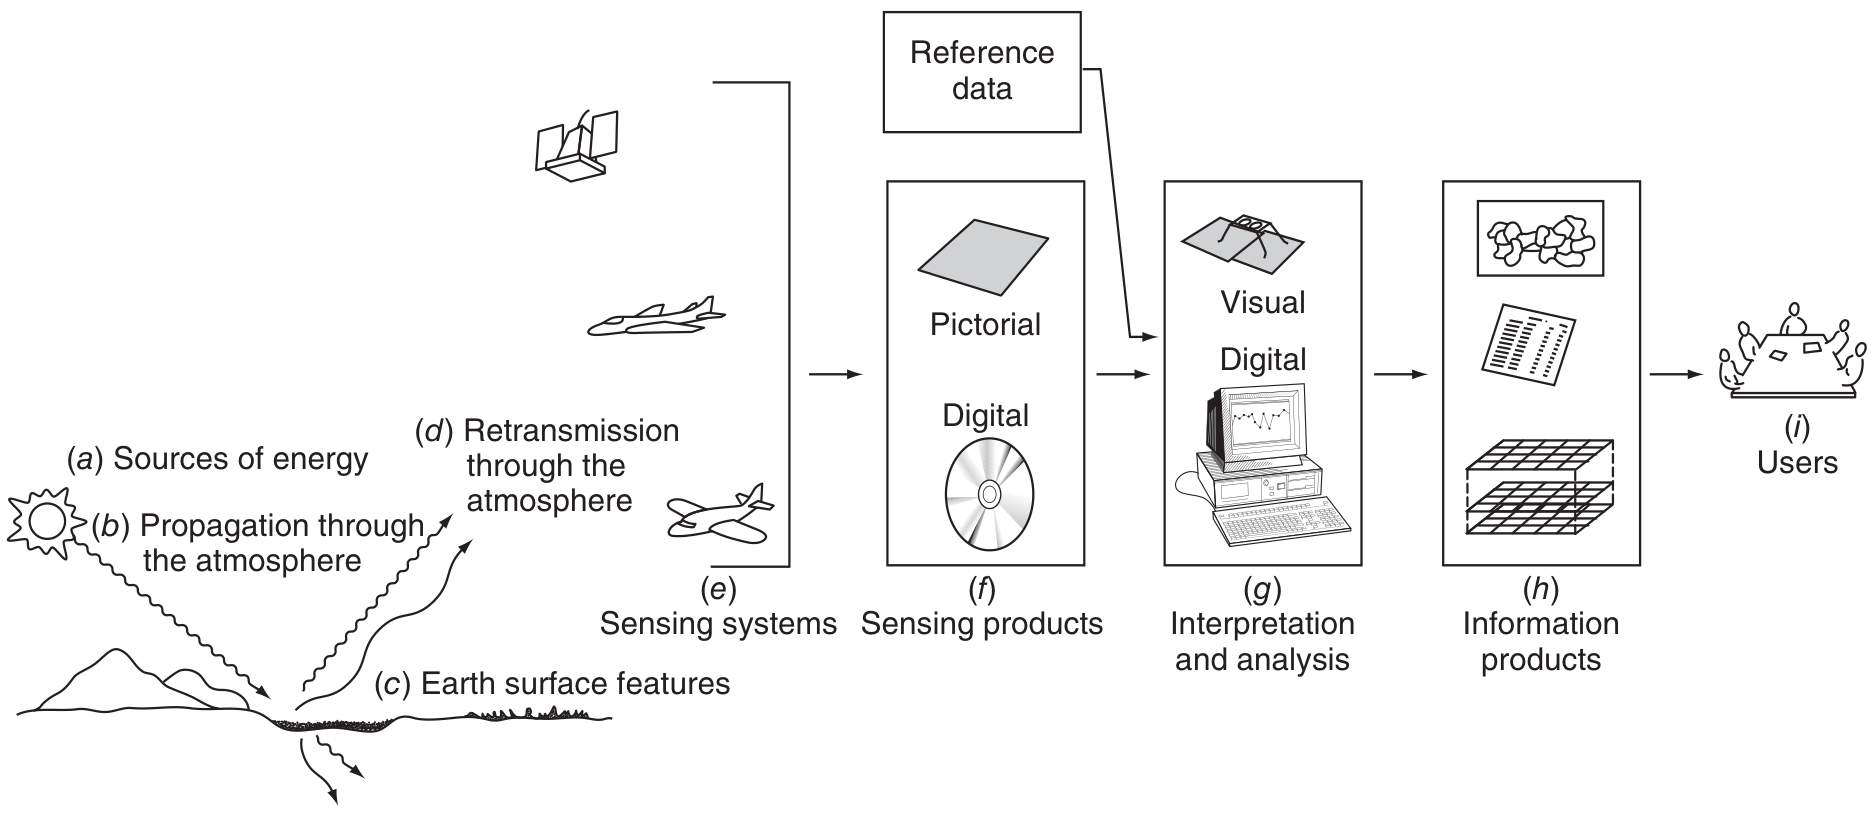
\includegraphics[width=0.88\linewidth]{../images/remote-sensing-of-electromagnetic-radiation-earth} \caption{Electromagnetic remote sensing of earth}\label{fig:electromagnetic-remote-sensing}
\end{figure}
\end{frame}

\begin{frame}{}
\protect\hypertarget{section-3}{}
\begin{itemize}
\tightlist
\item
  As developments in novel image processing algorithms and community
  around use and communication of image data continue, scientific value
  of remotely sensed data grow to the extent that never anticipated
  information are extracted.
\item
  However, there are tradeoffs between the local detail of the
  measurements (radiometric resolution, number of spectral bands) and
  the spatial scale of the area being measured.
\item
  Remote sensing is a more rapid means to sample multiple crop
  parameters from spectral indices such as NDVI.

  \begin{itemize}
  \tightlist
  \item
    Productive canopy surface (LAI)
  \item
    Productivity and yield potential
  \item
    Photosynthetic capacity
  \end{itemize}
\end{itemize}
\end{frame}

\begin{frame}{}
\protect\hypertarget{section-4}{}
\begin{figure}
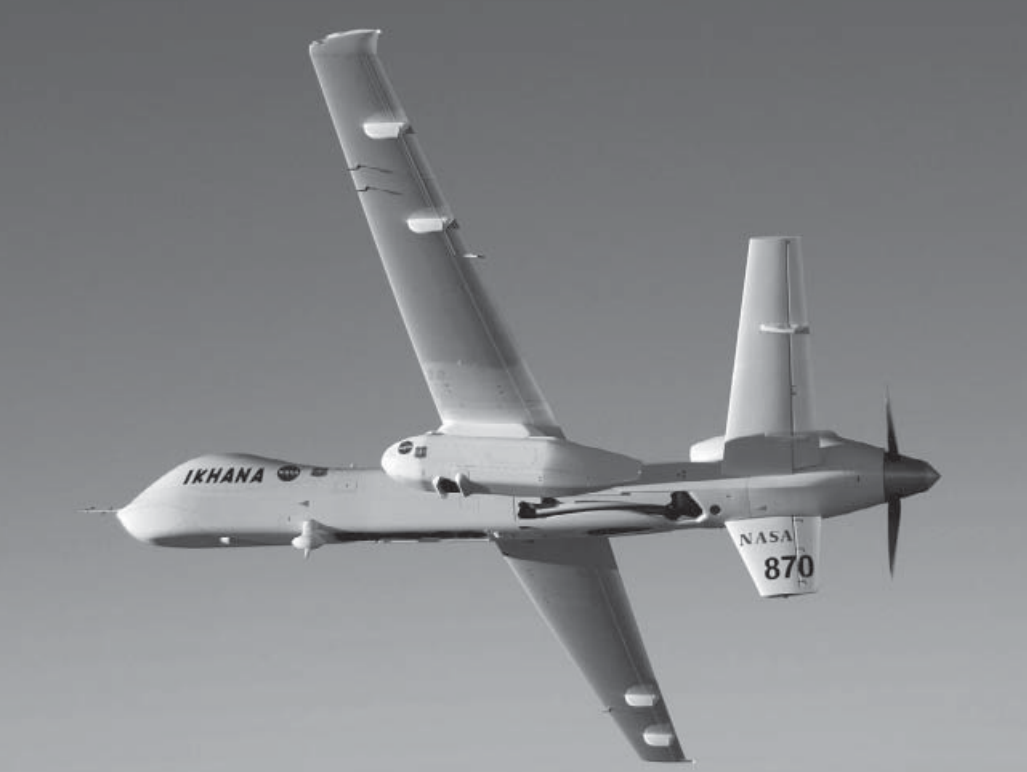
\includegraphics[width=0.65\linewidth]{../images/nasa_remote_sensing_uav} \caption{Uninhabited aerial vehicles (UAVs) used for environmental applications of remote sensing. (a) NASA’s Ikhana UAV, with imaging sensor in pod under left wing.}\label{fig:nasa-uav-remote-sensing}
\end{figure}
\end{frame}

\begin{frame}{Landsat imagery}
\protect\hypertarget{landsat-imagery}{}
\begin{itemize}
\tightlist
\item
  2022 marks 50th anniversary of the continuous planetary land coverage
  gathered by the Landsat imaging system.
\item
  Instruments on the Landsat satellites have acquired millions of images
  and can be viewed through the U.S. Geological Survey (USGS)
  ``EarthExplorer'' \footnote[frame]{https://earthexplorer.usgs.gov/}
  website.
\item
  Current version of the landsat (Landsat-9) was launched in September
  27, 2021
\item
  Currently Landsat program is managed jointly by:

  \begin{itemize}
  \tightlist
  \item
    NASA
  \item
    USGS
  \end{itemize}
\item
  Landsat 7 data has eight spectral bands with spatial resolutions
  ranging from 15 to 60 m (49 to 197 ft); the temporal resolution is 16
  days.
\item
  Landsat images are usually divided into scenes for easy downloading.
  Each Landsat scene is about 115 miles long and 115 miles wide (or 185
  kilometers long and 185 kilometers wide).
\item
  Landsat imagery is coarse in spatial resolution compared to using
  other remote sensing methods, such as imagery from airplanes.
\end{itemize}
\end{frame}

\begin{frame}{Applications of Landsat imagery}
\protect\hypertarget{applications-of-landsat-imagery}{}
\begin{itemize}
\tightlist
\item
  Agriculture risk management
\item
  Government mapping
\item
  Agricultural water use monitoring
\item
  Global security monitoring
\item
  Support for fire management
\item
  Detection of forest fragmentation
\item
  Detection of forest change
\item
  World agriculture supply and demand estimates
\item
  Vineyard management and water conservation
\item
  Flood mitigation mapping
\item
  Agricultural commodities mapping
\item
  Waterfowl habitat mapping and monitoring
\item
  Coastal change analysis
\item
  Forest health monitoring
\item
  Wildfire risk assessment
\item
  Fisheries, forestry, shrinking inland water bodies, fire damage,
  glacier retreat, urban development, and discovery of new species
\end{itemize}
\end{frame}

\begin{frame}{Image bands, resolution and features of Landsat}
\protect\hypertarget{image-bands-resolution-and-features-of-landsat}{}
\begin{table}

\caption{\label{tab:landsat-bands}Landsat 8 Operational Land Imager (OLI) and Thermal Infrared Sensor (TIRS). TIRS bands are acquired at 100 meter resolution, but are resampled to 30 meter in delivered data product}
\centering
\fontsize{8}{10}\selectfont
\begin{tabular}[t]{>{\raggedright\arraybackslash}p{14em}>{\raggedright\arraybackslash}p{10em}>{\raggedright\arraybackslash}p{10em}}
\toprule
Bands & Wavelength (micrometers) & Resolution (meters)\\
\midrule
Band 1 - Ultra Blue (coastal/aerosol) & 0.435 – 0.451 & 30\\
Band 2 - Blue & 0.452 – 0.512 & 30\\
Band 3 - Green & 0.533 – 0.590 & 30\\
Band 4 – Red & 0.636 – 0.673 & 30\\
Band 5 – NIR & 0.851 – 0.879 & 30\\
\addlinespace
Band 6 – SWIR 1 & 1.566 – 1.651 & 30\\
Band 7 – SWIR 2 & 2.107 – 2.294 & 30\\
Band 8 – Panchromatic & 0.503 – 0.676 & 15\\
Band 9 – Cirrus & 1.363 – 1.384 & 30\\
Band 10 – Thermal 1 & 10.60 – 11.19 & 100* (30)\\
\addlinespace
Band 11 – Thermal 2 & 11.50 – 12.51 & 100* (30)\\
\bottomrule
\end{tabular}
\end{table}
\end{frame}

\begin{frame}{}
\protect\hypertarget{section-5}{}
\begin{figure}
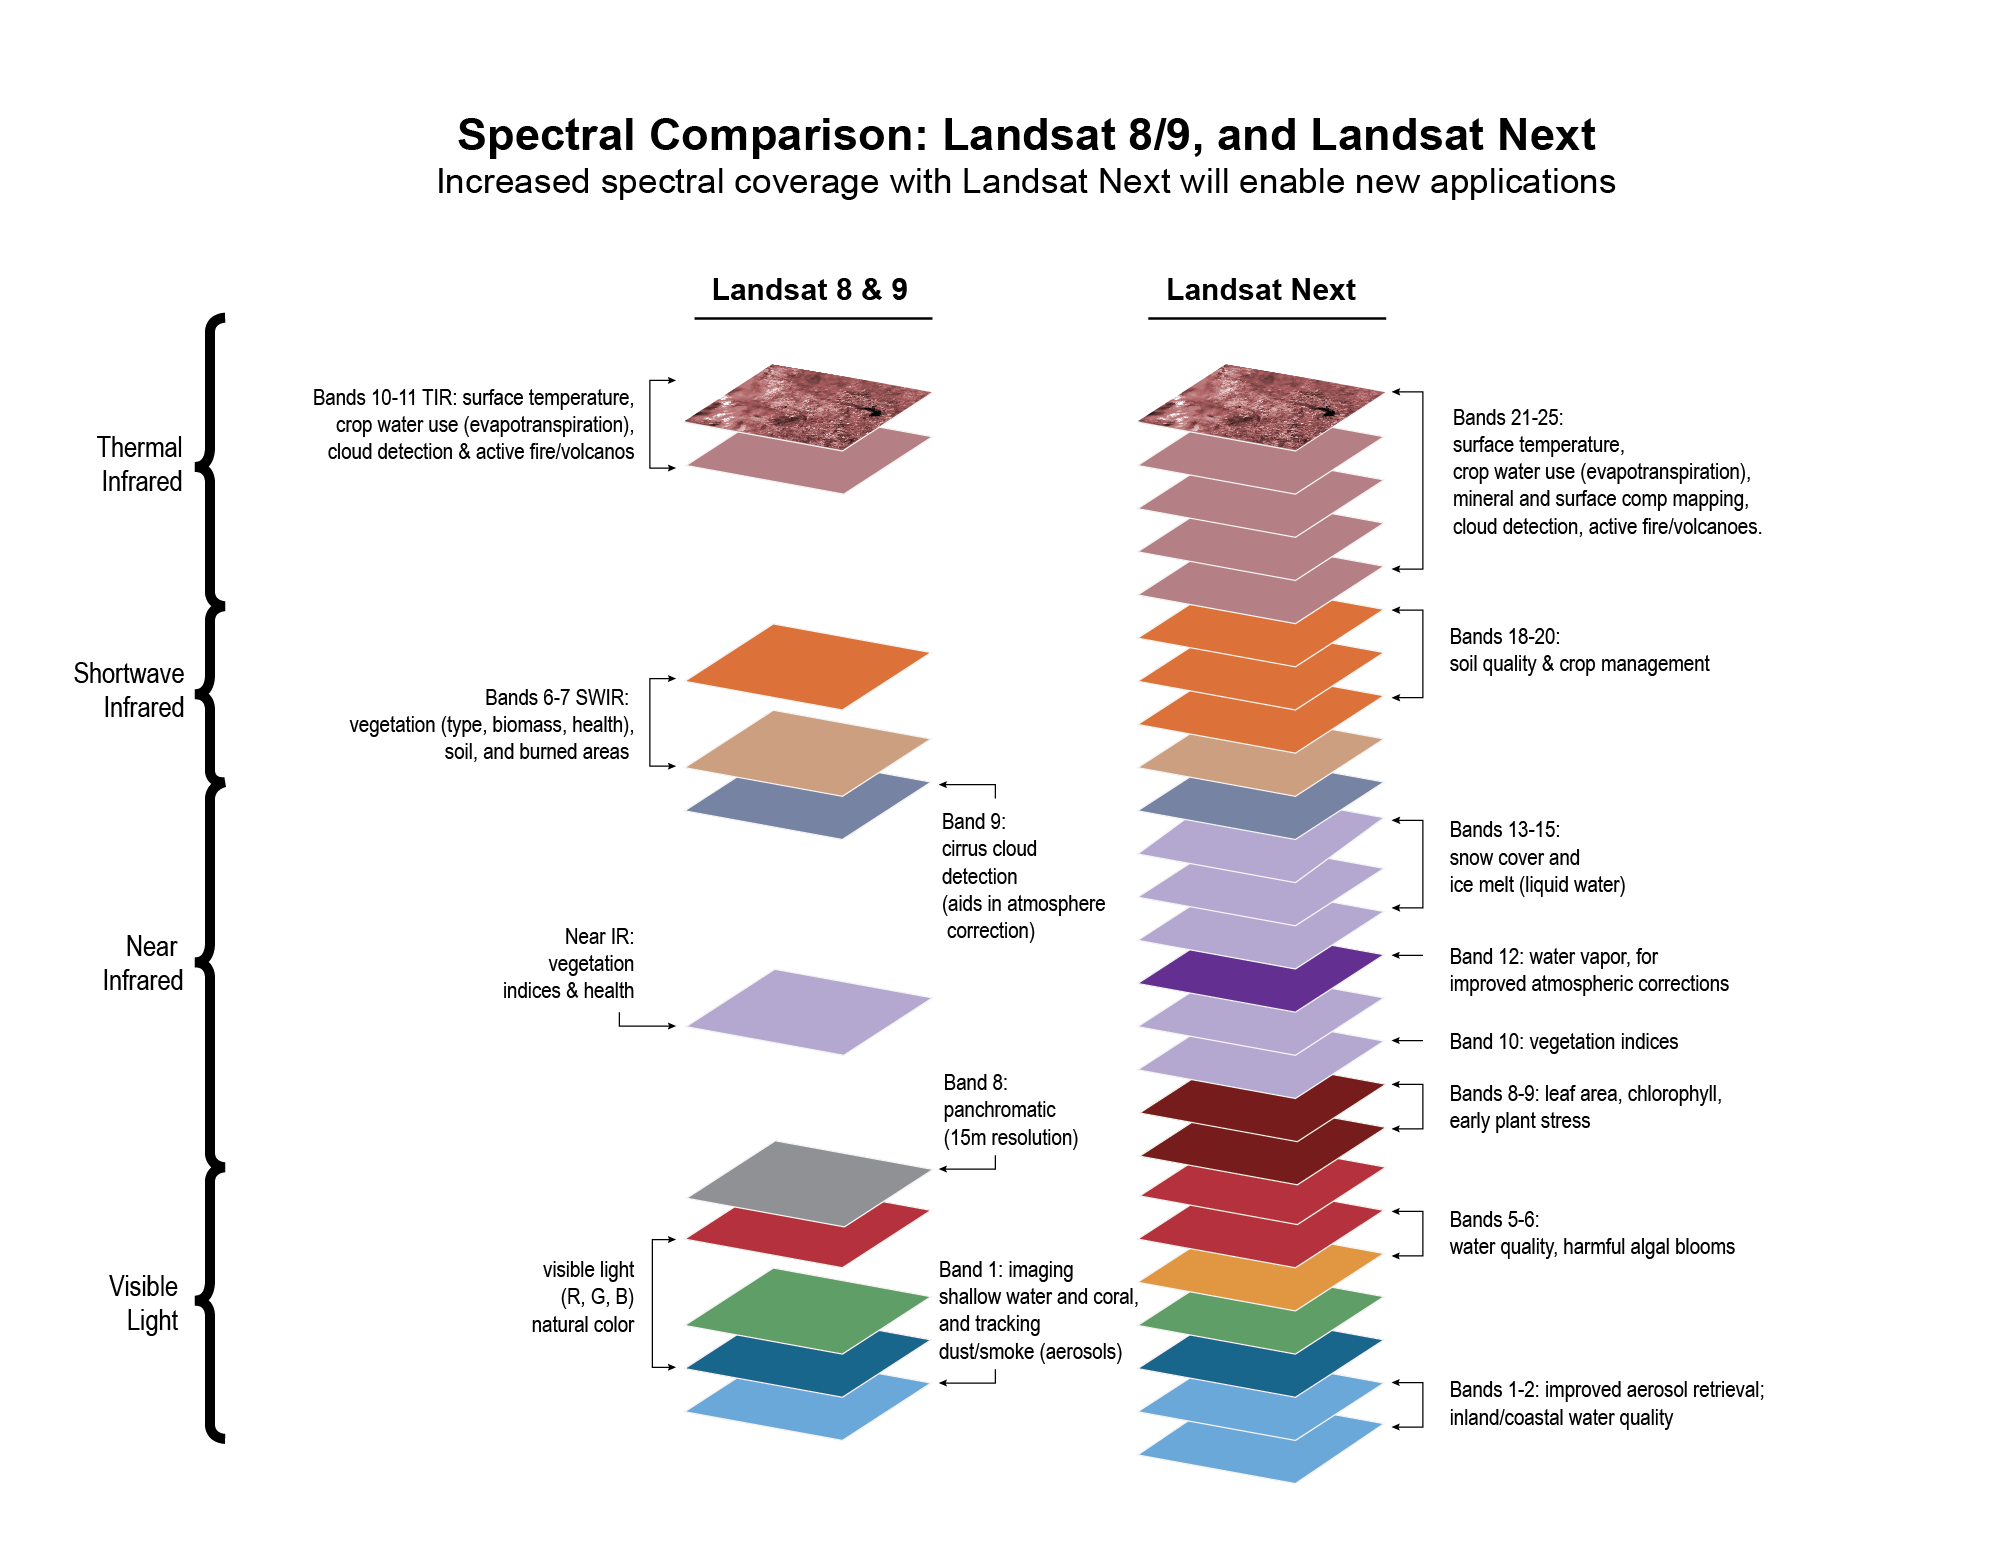
\includegraphics[width=0.65\linewidth]{../images/L8and9-to-LandsatNext-BandComparison} \caption{Source: \url{https://upload.wikimedia.org/wikipedia/commons/8/88/L8and9-to-LandsatNext-BandComparison.png}}\label{fig:band-comparison-lansat89-landsatnext}
\end{figure}
\end{frame}

\begin{frame}{Moderate Resolution Imaging Spectroradiometer (MODIS)}
\protect\hypertarget{moderate-resolution-imaging-spectroradiometer-modis}{}
\small

\begin{itemize}
\tightlist
\item
  An imaging sensor built by Santa Barbara Remote Sensing that was
  launched into Earth orbit by NASA in 1999 on board the Terra (EOS AM)
  satellite, and in 2002 on board the Aqua (EOS PM) satellite.

  \begin{itemize}
  \footnotesize
  \item Wide spectral band
  \item High frequency and temporal coverage
  \end{itemize}
\item
  Instrument captures data of 36 spectral bands and has a 2330 km wide
  viewing swath, seeing every point on earth every 1-2 days.
\item
  Mostly useful for measuring atmospheric variables, including cloud
  cover, the size of cloud droplets in both liquid water and ice
  particles, aerosols and pollution from natural and man-made sources
  like industry emissions, dust storms, volcanic eruptions and forest
  fires.
\end{itemize}
\end{frame}

\begin{frame}[fragile]{Data description -- Metadata}
\protect\hypertarget{data-description-metadata}{}
\begin{figure}
\begin{columns}[T,onlytextwidth]

  \column{.6\linewidth}
  \begin{center}
  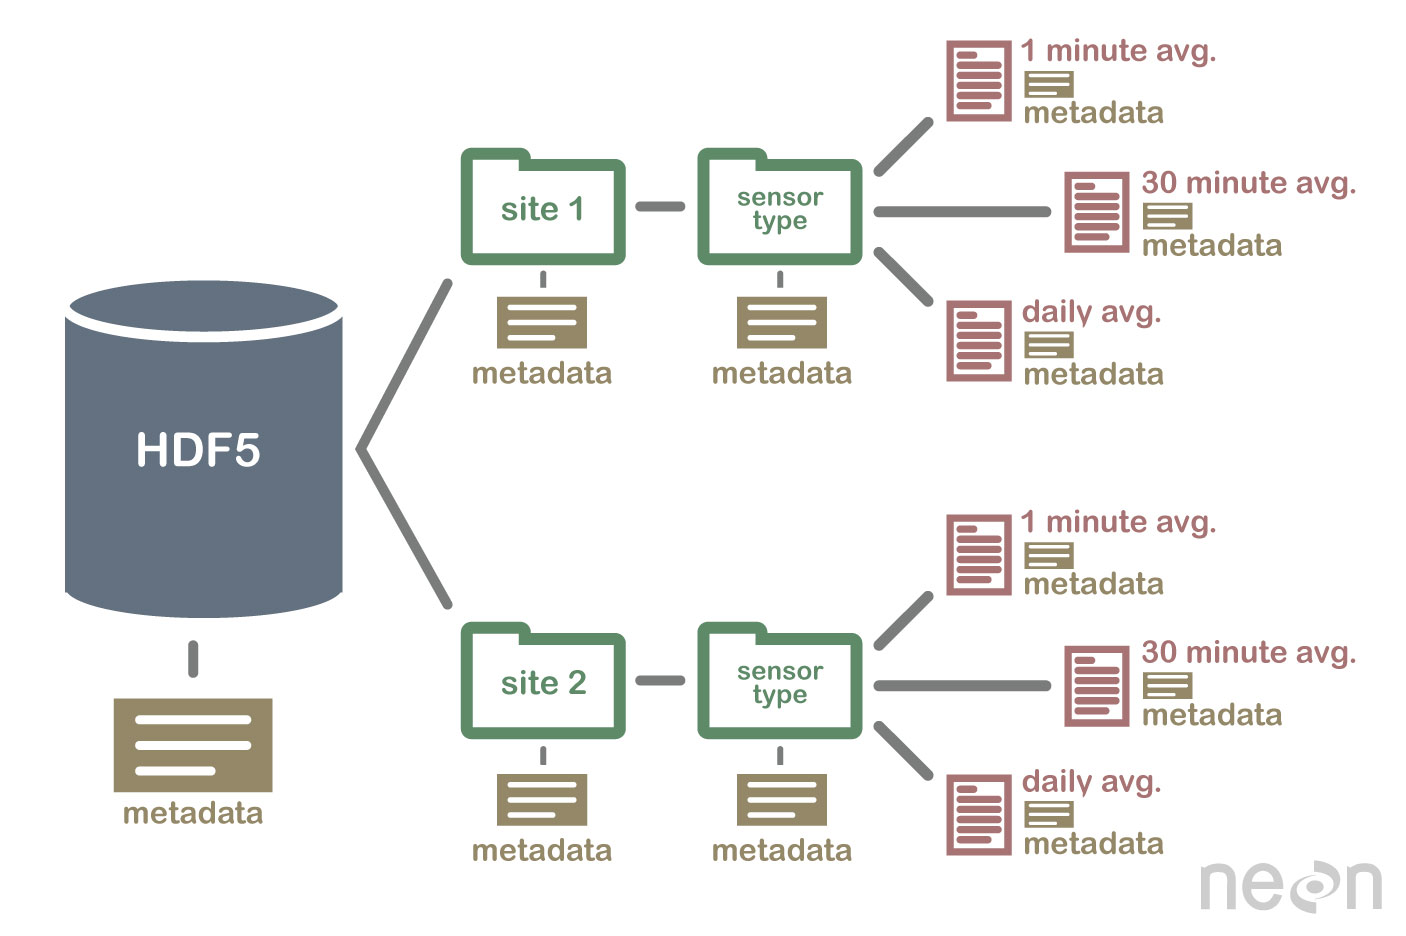
\includegraphics[width=0.30\linewidth]{../images/2020-09-01-MODIS-hdf-file-info.jpg}
  \end{center}
  
  \column{.4\linewidth}
  \caption{\newline HDF files are self describing. All elements (the file itself, groups and datasets) can have associated meta-data that describes the information contained within the element.}
  \label{fig:metadata-modis}
  
  \end{columns}
\end{figure}

\begin{figure}
\begin{columns}[T,onlytextwidth]

  \column{.7\linewidth}
  \begin{center}
  \includegraphics[width=0.85\linewidth]{../images/MCD43D09.A2022310.006.2022322075329_south_asia_focus_albedo.png}
  \end{center}
  
  \column{.3\linewidth}
  \caption{\newline Bidirectional Reflectance Distribution Function and Albedo (BRDF/Albedo) Model Parameter dataset (clipped to display South Asian region) is produced daily using 16 days of Terra and Aqua Moderate Resolution Imaging Spectroradiometer (MODIS) data at 30 arc second (1,000 meter) resolution. The pixels represented in binary are infact derived from unscaled values (by QGIS).}
  \label{fig:modis-albedo-layer}
  
  \end{columns}
\end{figure}

\begin{verbatim}
# An HDF file contains layers of raster with spectral bands, meta information and CRS.

# To access HDF, you can use 3 different R packages.
# 
# ncdf4: This package works for both HDF4 and HDF5. (Might needs to be built using source? For help and troubleshooting refer to: https://hdfeos.org/software/r.php)
# rgdal: This package works for both HDF4 and HDF5. This is convenient for datasets that have the characteristics of raster images and for data conversion between HDF and GeoTIFF.
# h5: This package works only for HDF5.

# Since the file sizes are large, better not import the hdf files in R.
# but import in QGIS and export in print layout format
# for a file (MCD43D09.A2022310.006.2022322075329.hdf) rendered in print layout using QGIS, following is layer information

# SDS name: Global_BRDF_Albedo_Parameter3_Band3
# Description: BRDF model parameter for geo kernel of band 3
# Units: N/A
# Data type: 16-bit signed integer
# Fill value: 32767
# No data value: N/A
# Valid range: 0 to 32766
# Scale factor: 0.001

# The MCD43D09 Version 6 Bidirectional Reflectance Distribution Function and Albedo (BRDF/Albedo) Model Parameter dataset is produced daily using 16 days of Terra and Aqua Moderate Resolution Imaging Spectroradiometer (MODIS) data at 30 arc second (1,000 meter) resolution. Data are temporally weighted to the ninth day which is reflected in the Julian date in the file name. This Climate Modeling Grid (CMG) product covers the entire globe for use in climate simulation models. Due to the large file size, each MCD43D product contains just one data layer. Each of the three model parameters (isotropic, volumetric, and geometric) for each of the MODIS bands 1 through 7 and the visible, near-infrared (NIR), and shortwave bands included in MCD43C1 are stored in a separate file as MCD43D01 through MCD43D30.
# 
# MCD43D09 is the BRDF geometric parameter for MODIS band 3. The geometric parameter, in conjunction with the isotropic and volumetric parameters, is used to derive the BRDF/Albedo values for MODIS band 3.

# Collection
# Characteristic    Description
# Collection    Combined MODIS
# DOI   10.5067/MODIS/MCD43D09.006
# File Size ~134.4 MB
# Temporal Resolution   Daily
# Temporal Extent   2000-02-16 to Present
# Spatial Extent    Global
# Coordinate System Geographic Latitude and Longitude
# Datum N/A
# File Format   HDF-EOS
# Geographic Dimensions Global

# Granule
# Characteristic    Description
# Number of Science Dataset (SDS) Layers    1
# Columns/Rows  43200 x 21600
# Pixel Size    ~1000 m
\end{verbatim}
\end{frame}

\hypertarget{acquiring-remotely-sensed-data}{%
\section{Acquiring remotely sensed
data}\label{acquiring-remotely-sensed-data}}

\begin{frame}{Landsat Missions of USGS}
\protect\hypertarget{landsat-missions-of-usgs}{}
\begin{columns}[T, onlytextwidth]

\column{0.5\textwidth}


\begin{center}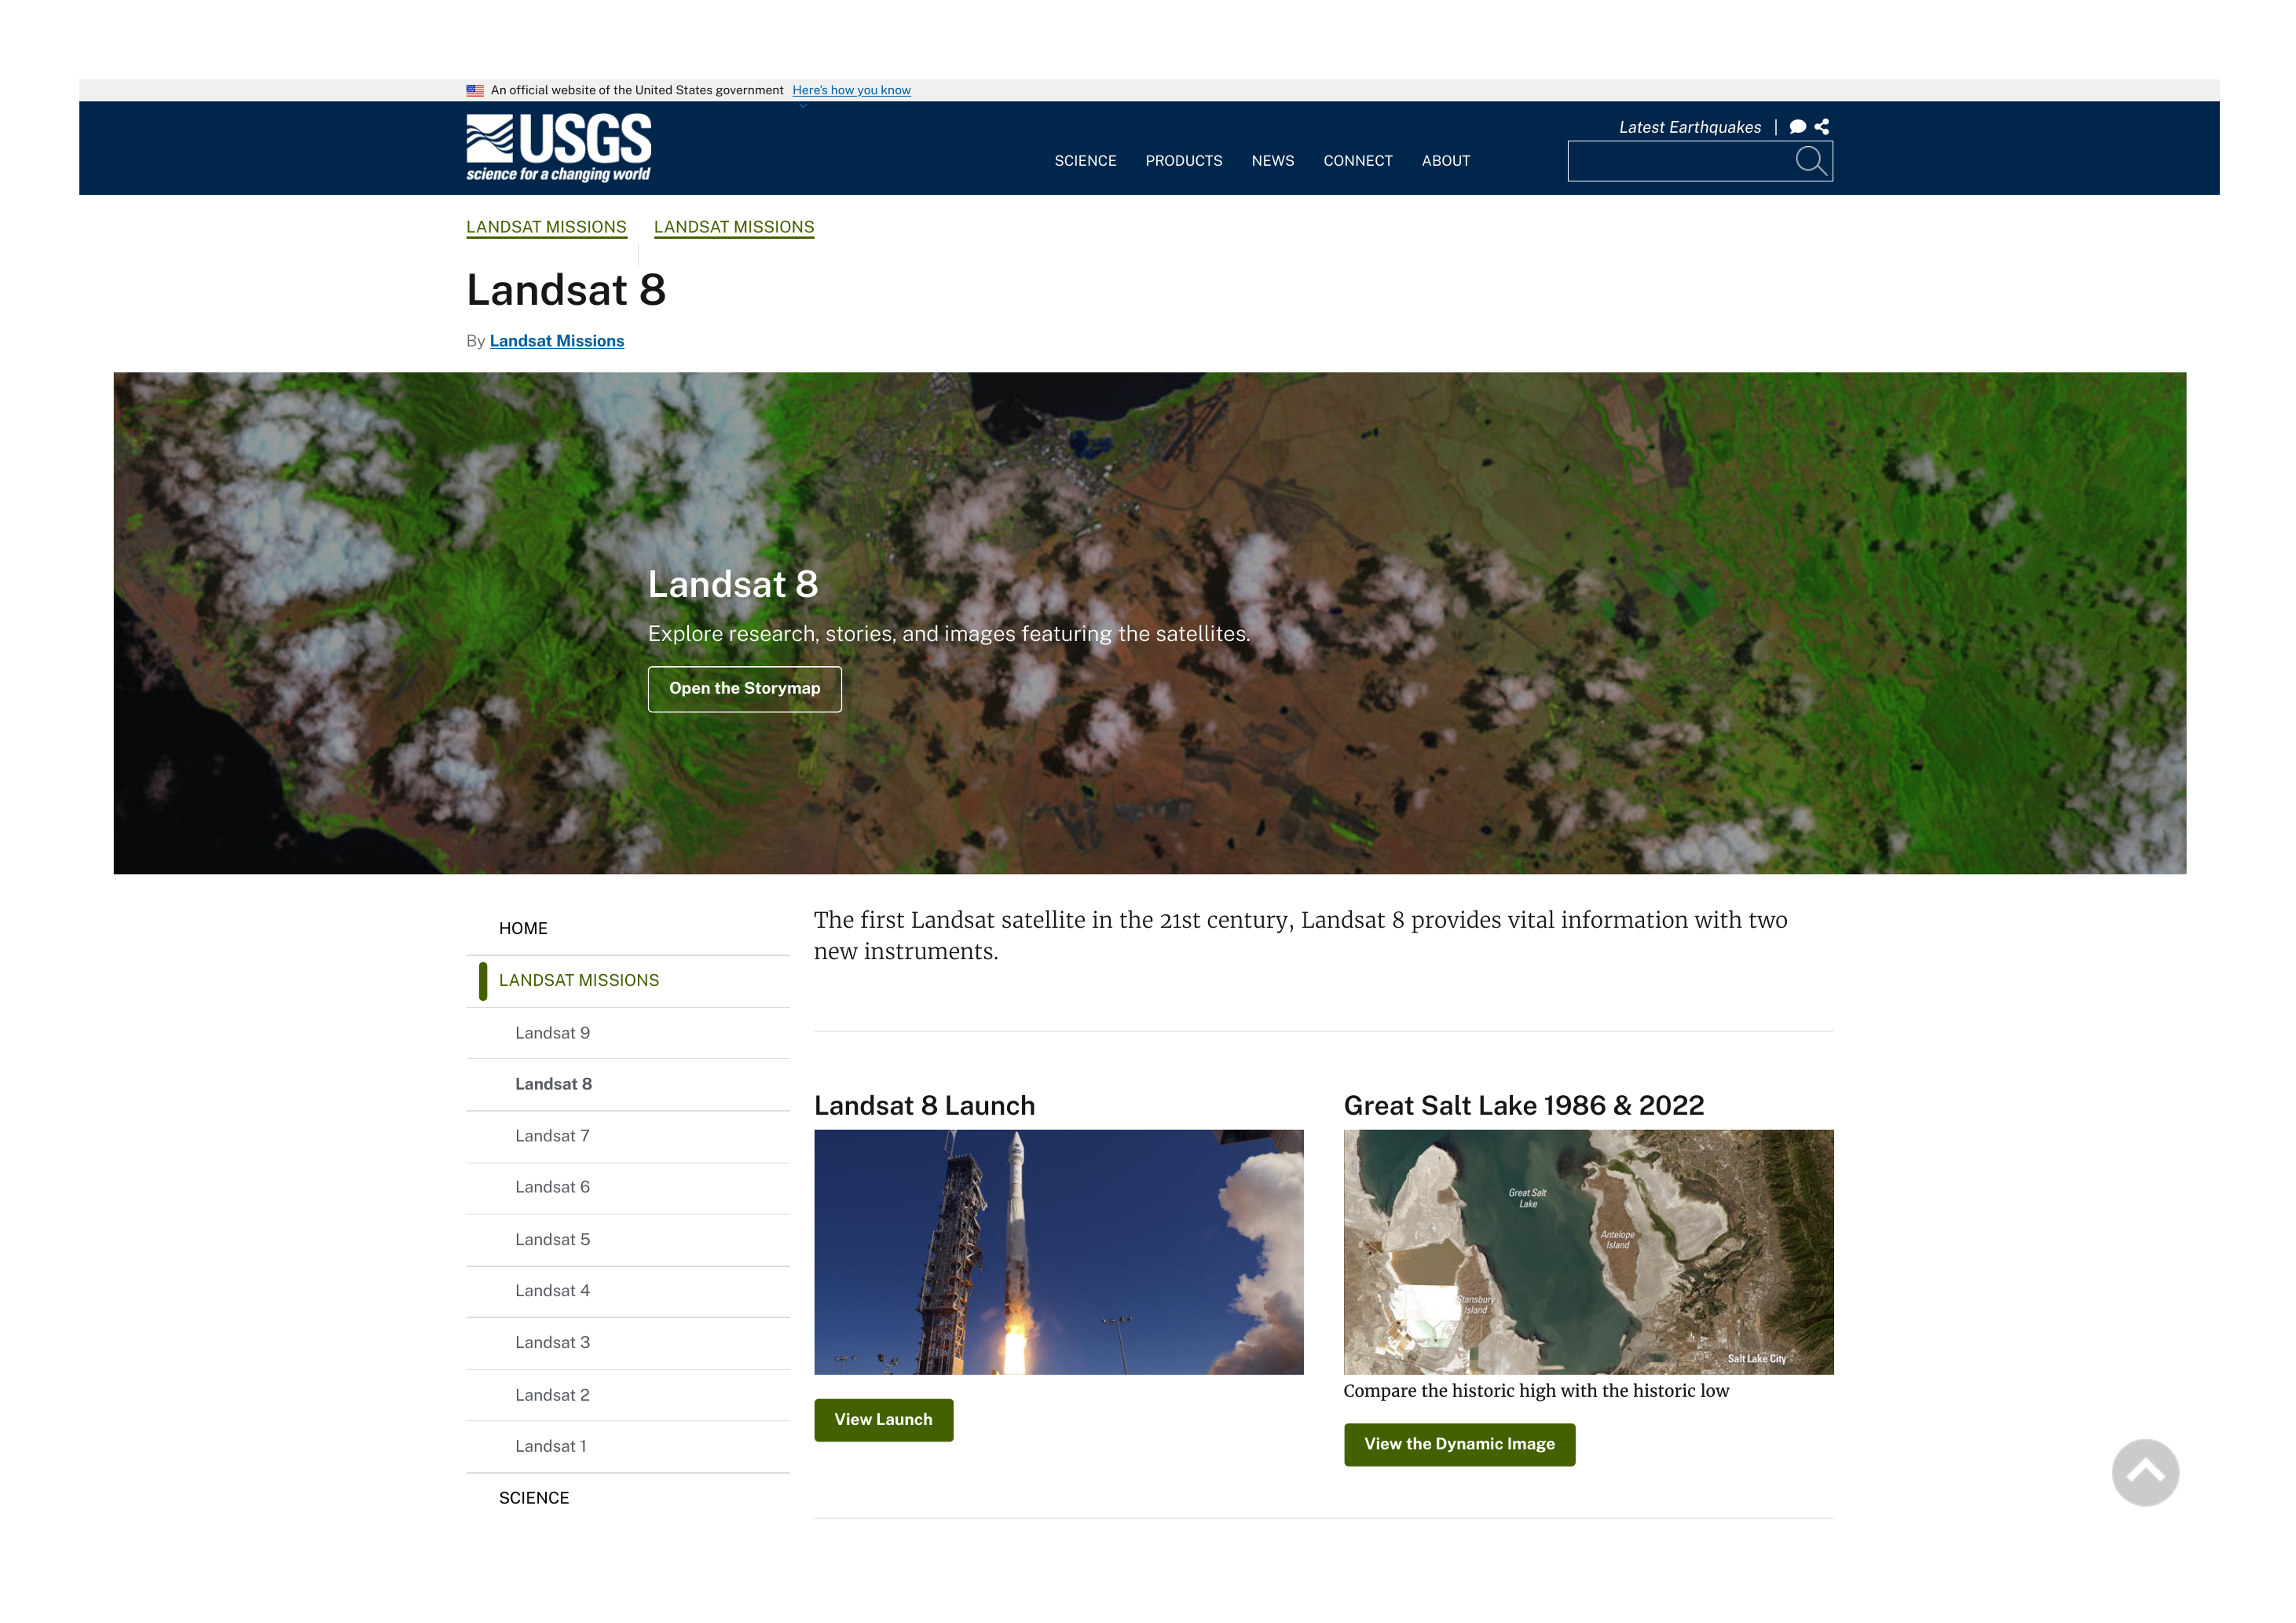
\includegraphics[width=0.98\linewidth]{../images/usgs_official_portal_p1} \end{center}

\column{0.5\textwidth}



\begin{center}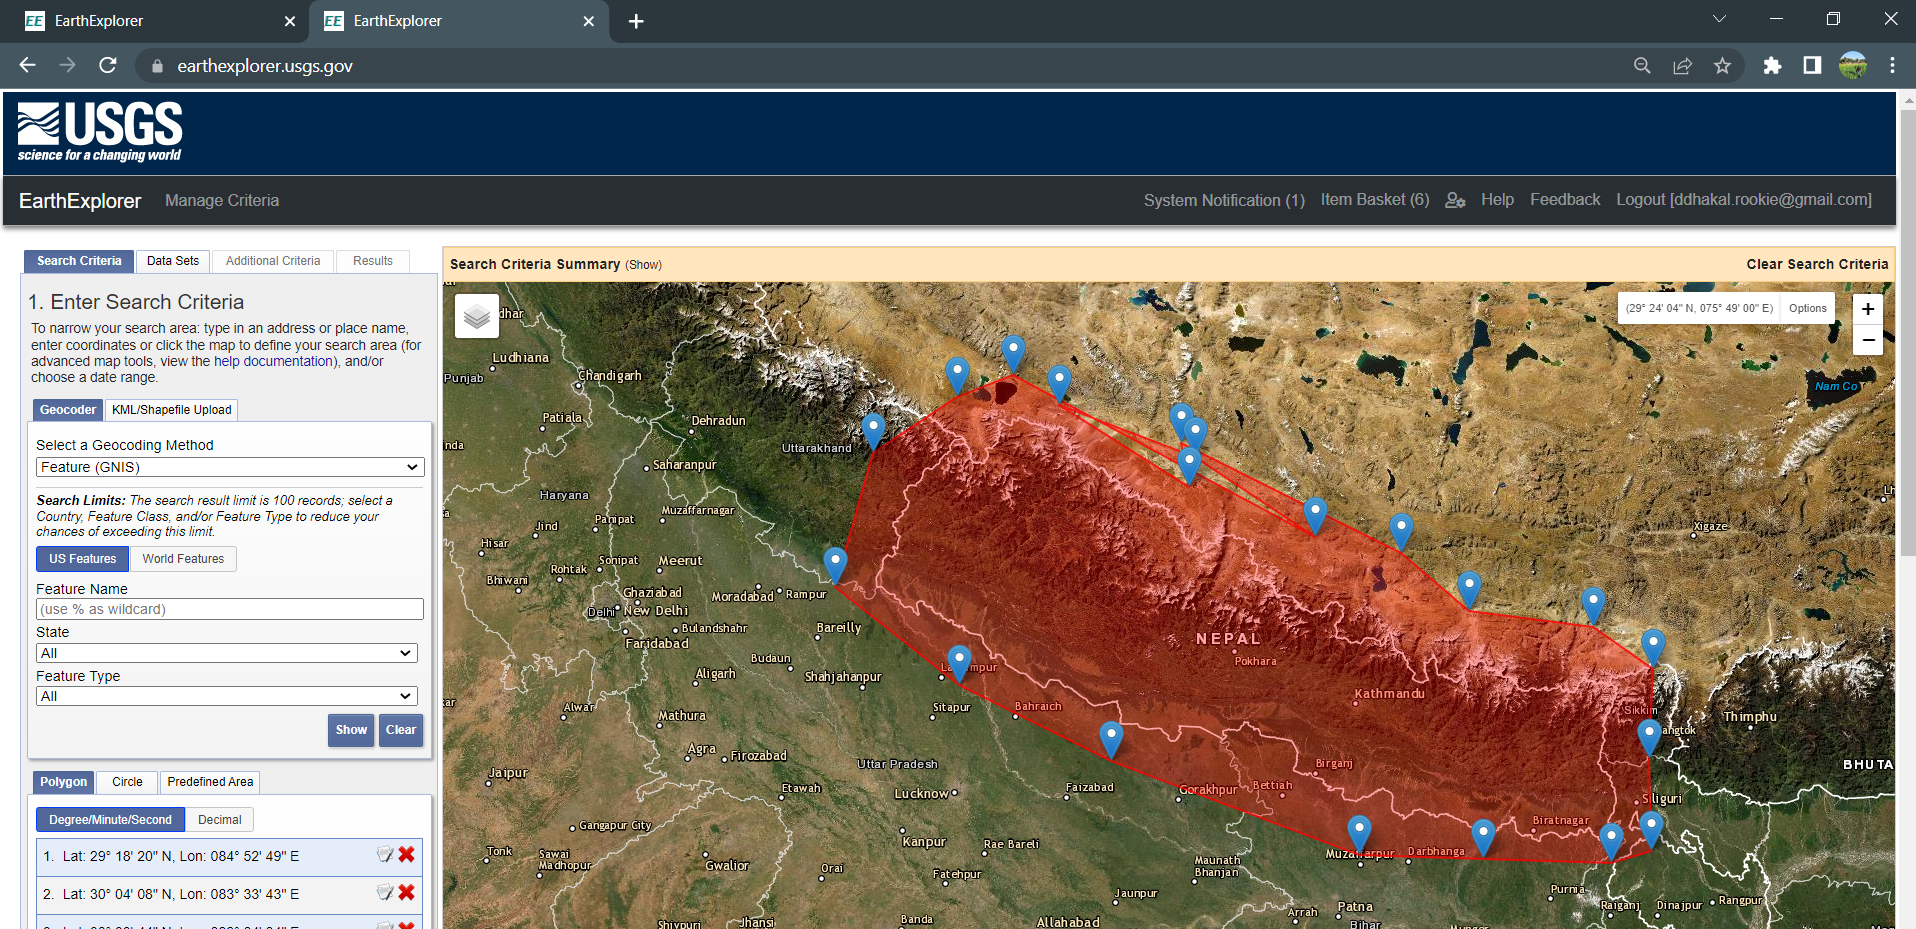
\includegraphics[width=0.98\linewidth]{../images/usgs_landsat_mapping_earth_explorer} \end{center}

\end{columns}
\end{frame}

\begin{frame}{Sentinel mission of NASA}
\protect\hypertarget{sentinel-mission-of-nasa}{}
\begin{center}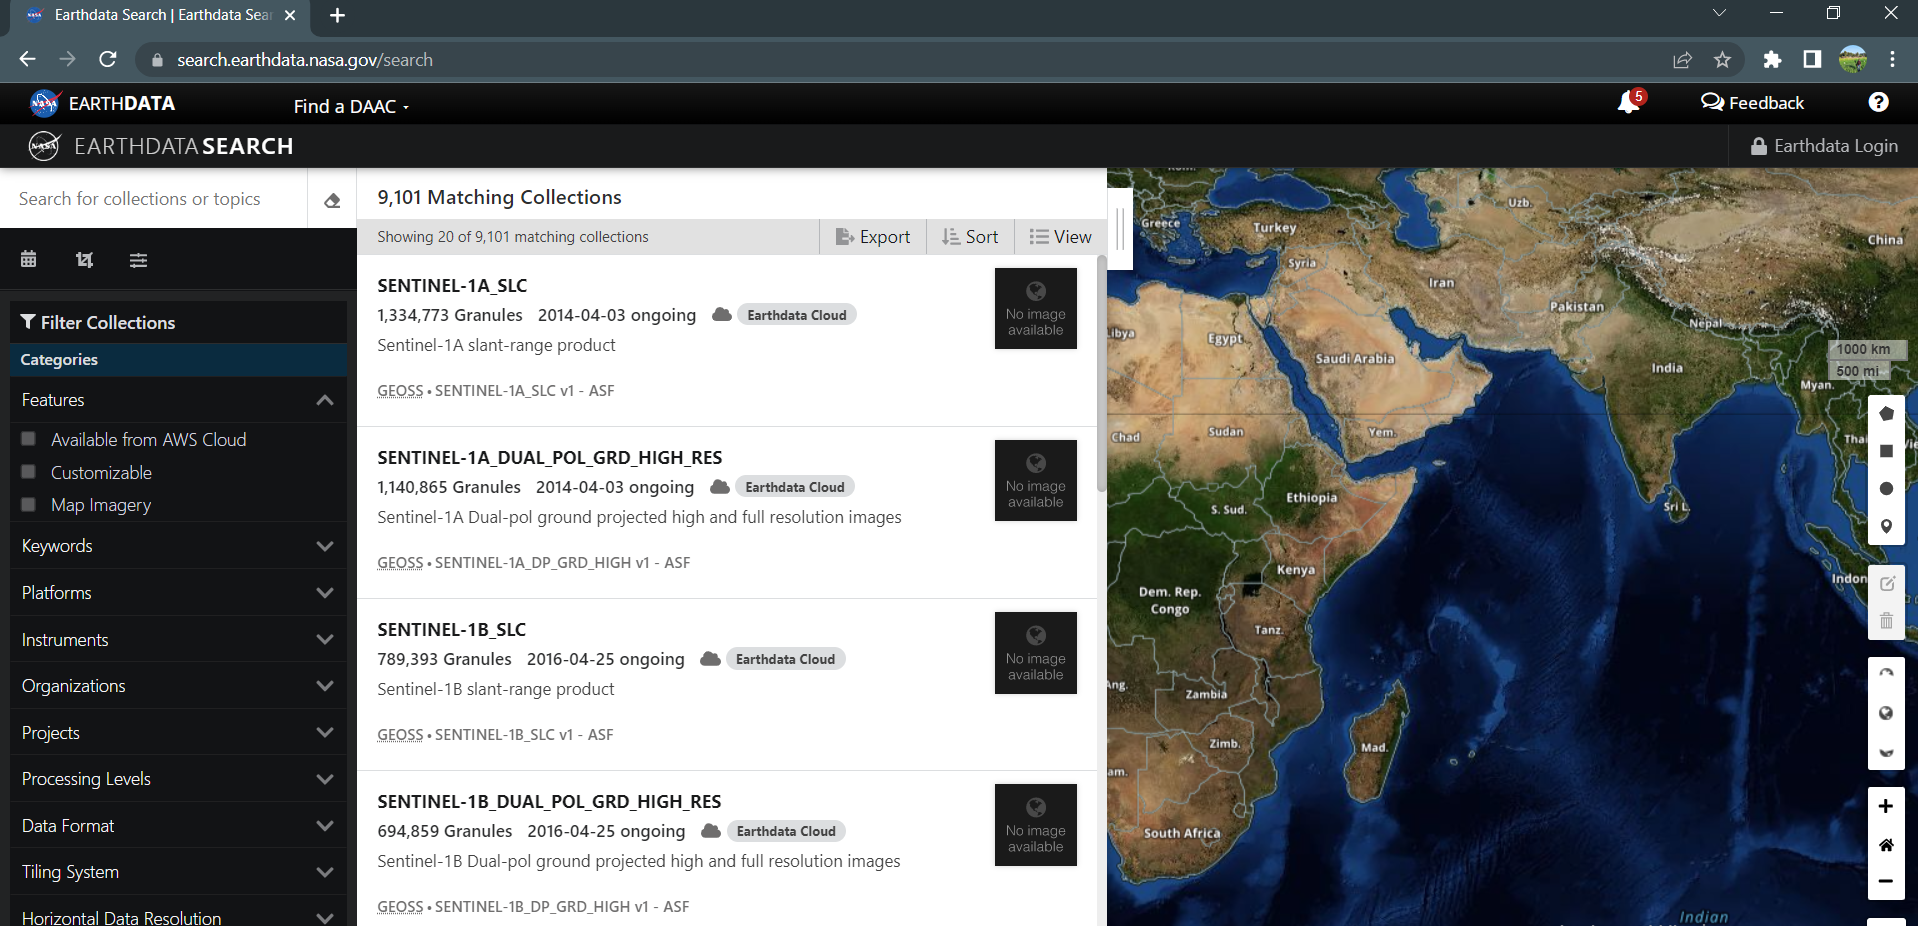
\includegraphics[width=0.85\linewidth]{../images/earthdata_nasa_sentinel_data_viewer} \end{center}
\end{frame}

\hypertarget{image-and-use-of-photographic-image-in-scene-measurement}{%
\section{Image and use of photographic image in scene
measurement}\label{image-and-use-of-photographic-image-in-scene-measurement}}

\begin{frame}{Image}
\protect\hypertarget{image}{}
\begin{block}{Casual definition}
Is a visual representation of something. It can be two-dimensional, three-dimensional, or somehow otherwise feed into the visual system to convey information.
\end{block}

\begin{block}{Mathematical definition}
An image is a two-dimensional function f(x, y), where x and y are the spatial (plane) coordinates, and the amplitude of f at any pair of coordinates (x, y) is called the intensity of the image at that level.
\end{block}

\begin{description}
\item[Digital image] If x, y and the amplitude values of f are finite and discrete quantities, we call the image a digital image. A digital image is composed of a finite number of elements called pixels, each of which has a particular location and value.
\end{description}
\end{frame}

\begin{frame}{}
\protect\hypertarget{section-6}{}
\begin{itemize}
\tightlist
\item
  An image is generic term for any pictorial representation of data.

  \begin{itemize}
  \tightlist
  \item
    a pictorial record from a ``thermal scanner'' (electronic scanner)
    would be called a ``thermal image.''
  \end{itemize}
\item
  Not all images are photographs. (Try calling a `thermal image' a
  `thermal photograph!')
\item
  Spectral characteristics are not always fully evaluated in visual
  interpretation efforts because of the limited ability of the eye to
  discern tonal values on an image and the difficulty of simultaneously
  analyzing numerous spectral images.
\item
  In applications where spectral patterns are highly informative, it is
  therefore preferable to analyze digital, rather than pictorial.
\end{itemize}
\end{frame}

\begin{frame}{Image acquisition}
\protect\hypertarget{image-acquisition}{}
\scriptsize

\begin{itemize}
\tightlist
\item
  Images are generated by the combination of an
  \alert{illumination source} and the reflection or absorption of energy
  from that source by the elements of the \alert{scene} being imaged.
\item
  Imaging sensors are used to transform the illumination energy into
  digital images.
\end{itemize}

\begin{figure}
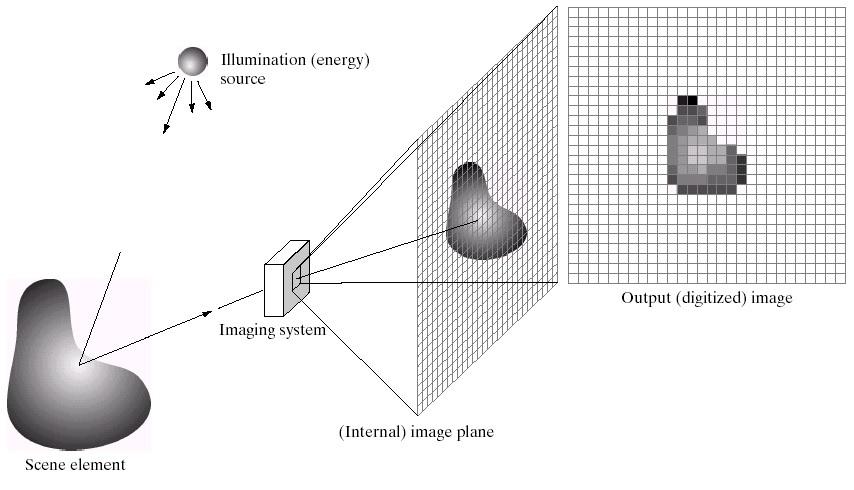
\includegraphics[width=0.6\linewidth]{../images/generation_of_digital_image} \caption{An example of the digital image acquisition process. Stages: (a) Energy ('illumination') source. (b) An element of a scene. (c) Imaging system. (d) Projection of the scene onto the image plane. (e) Digitized image.}\label{fig:imaging-sensors}
\end{figure}
\end{frame}

\begin{frame}{Area calculation}
\protect\hypertarget{area-calculation}{}
\begin{itemize}
\tightlist
\item
  Process of measuring areas using aerial photographs can be
  accomplished in many ways.
\item
  Accuracy of area measurement is a function of not only the measuring
  device used, but also the degree of image scale variation due to
  relief in the terrain and tilt in the photography.

  \begin{itemize}
  \tightlist
  \item
    accurate measurements are obtained from vertical photos of areas of
    low relief
  \end{itemize}
\item
  Simple scales may be used to measure the are of simply shaped features

  \begin{itemize}
  \tightlist
  \item
    area of a rectangular field can be determined by simply measuring
    its length and width
  \item
    area of circular feature can be computed after measuring its radius
    or diameter
  \end{itemize}
\end{itemize}
\end{frame}

\begin{frame}{}
\protect\hypertarget{section-7}{}
\textbf{Numerical problem}

A rectangular agricultural field measures 8.65 cm long and 5.13 cm wide
on a vertical photograph having a scale of 1:20000. Find the area of the
field at ground level.

\(\longrightarrow\)

\(\text{Ground length} = \text{Photo length} \times \frac{1}{S} = 0.0865 m \times 20,000 = 1730 m\)

\(\text{Ground width} = \text{Photo width} \times \frac{1}{S} = 0.0513 m \times 20,000 = 1026 m\)

\(\text{Ground area} = 1730m \times 1026m = 1,774,980m^2 = 177 ha\)
\end{frame}

\begin{frame}{}
\protect\hypertarget{section-8}{}
\bcolumns
\column{0.5\textwidth}
\footnotesize

\begin{itemize}
\tightlist
\item
  For measuring irregularly shaped features, a simplest technique uses
  transparent grid overlay consisting of lines forming rectangles or
  squares of known area.
\item
  The grid is placed over the photograph and the area of a ground unit
  is estimated by counting the number of grid units that fall within the
  unit to be measured.
\end{itemize}

\begin{figure}
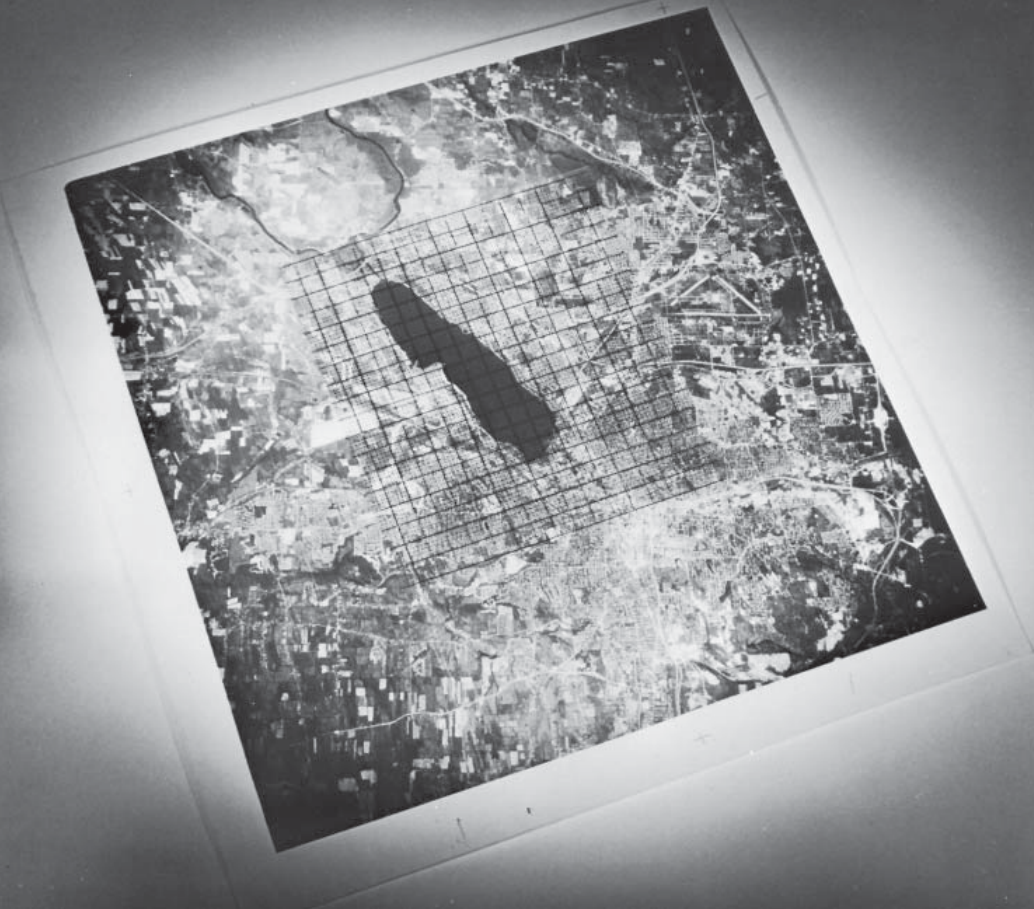
\includegraphics[width=0.7\linewidth]{../images/transparent_dot_grid_overlay} \caption{Transparent dot grid overlay.}\label{fig:transparent-dot-grid}
\end{figure}

\column{0.5\textwidth}

\footnotesize

\textbf{Numerical problem}

A flooded area is covered by 129 dots on a \(25\mathrm{-dot/cm^2}\) grid
on a 1:20,000 vertical aerial photograph. Find the ground area flooded.

\(\longrightarrow\)

\(\text{Dot density} = \frac{\mathrm{1~cm^2}}{\mathrm{25~dots}} = 16,000,000 \mathrm{~cm^2/dot} = 0.16 \mathrm{~ha/dot}\)

\(\text{Ground area} = 129\mathrm{~dots} \times 0.16 \mathrm{~ha/dot} = 20.6\mathrm{~ha}\)

\ecolumns
\end{frame}

\hypertarget{image-processing}{%
\section{Image processing}\label{image-processing}}

\begin{frame}{}
\protect\hypertarget{section-9}{}
\begin{figure}
  \begin{columns}[T,onlytextwidth]
  \column{.8\linewidth}
  \begin{center}
  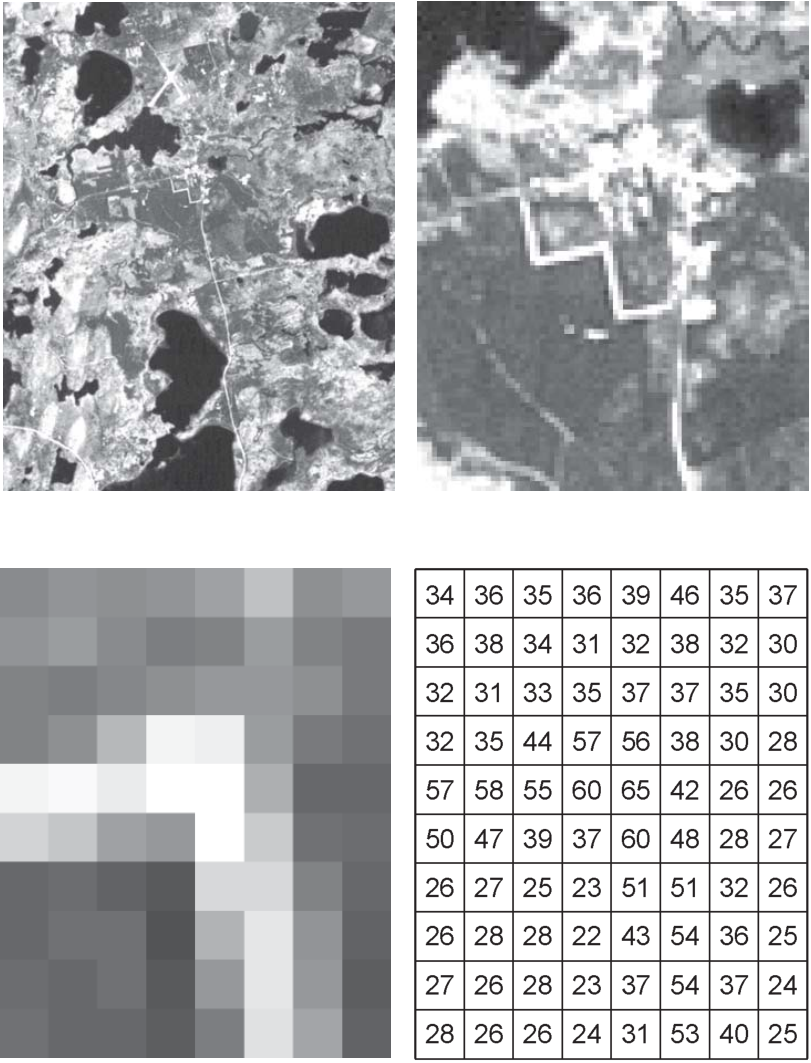
\includegraphics[width=0.48\linewidth]{../images/features_of_digital_image.PNG}
  \end{center}
  
  \column{.2\linewidth}
  \caption{\newline\tiny The image shown in upper left is actually composed of a two-dimensional array of discrete picture elements, or pixels. They intensity of each pixel corresponds to the average brightness, or radiance, measured electronically over the ground area corresponding to each pixel. A total of 500 rows and 400 columns of pixels are shown. Whereas the individual pixels are virtually impossible to discern in first image, they are readily observable in the enlargements shown in upper right (100 row x 80 column) and lower left (10 row x 8 column). These enlargements correspond to sub-areas located near the center of the first image. In the lower right is shown the individual \textit{digital number (DN)} also referred to as 'brightness value' or 'pixel value' -- corresponding to the average radiance measured in each pixel shown on the left. These values result from quantizing the original signal from the sensor into positive integer values using a process called 'analog-to-digital (A-to-D) signal conversion'.}
  \label{fig:features-digital-image}
  
  \end{columns}
\end{figure}
\end{frame}

\begin{frame}{Preprocessing}
\protect\hypertarget{preprocessing}{}
\begin{itemize}
\tightlist
\item
  To remove noise and increase the interpretability of image data
  (essential when a time series of imagery is used or when when multiple
  image operation such as join is required to account for an area
  encompassed by many images to make these images compatible spatially
  and spectrally)
\item
  All images after image preprocessing should appear as if they were
  acquired from the same sensor (Hall et al.~1991).
\item
  Image processing sensors are usually categorized into levels (0, 1A,
  1B, 2A, 2B, 3A, 3B with image quality gradually increased). For
  example, for most sensors, level 3A means that radiometric correction,
  geometric correction and orthorectification have been processed for
  the images.
\item
  Factors such as seasonal phenology, ground conditions and atmospheric
  conditions can contribute to variability in multi-temporal spectral
  responses that may have little to do with the remote sensed objects
  themselves (Song and Woodcock 2003)
\end{itemize}
\end{frame}

\begin{frame}{}
\protect\hypertarget{section-10}{}
\begin{itemize}
\tightlist
\item
  Image preprocessing commonly comprises a series of operations,

  \begin{itemize}
  \tightlist
  \item
    including but not limited to bad lines replacement,
  \item
    radiometric correction,
  \item
    geometric correction,
  \item
    image enhancement and masking (e.g.~for clouds, water, irrelevant
    features) although variations may exist for images acquired by
    different sensors.
  \item
    bad line replacement (fills in missing lines with the line above,
    below or with an average of the two) to determine the overall
    quality of the images (e.g.~missing data lines) through visually
    previewing the images band-by-band
  \item
    cloud imposes a big noise in mapping vegetation cover for
    identifying and thus has to be removed or masked.

    \begin{itemize}
    \tightlist
    \item
      neural network to detect cloud in SPOT VEGETATION images
    \item
      cloud-free space shuttle photograph to detect and remove (mask)
      unwanted cloud covers in Landsat TM scenes
    \end{itemize}
  \end{itemize}
\end{itemize}
\end{frame}

\begin{frame}{Image pre-processing: Radiometric correction}
\protect\hypertarget{image-pre-processing-radiometric-correction}{}
\begin{itemize}
\tightlist
\item
  radiometric correction normally involves the process of correcting
  radiometric errors or distortions of digital images to improve the
  fidelity of the brightness values. radiometric correction methods
  (absolute and relative correction):

  \begin{itemize}
  \tightlist
  \item
    complex mathematical models that describe the main interactions
    involved (certain parameters (i.e.~the atmospheric composition) must
    be known before applying them).
  \item
    methods based on the observations of reference targets (e.g.~water
    or desert land) whose radiometry is known.
  \end{itemize}
\end{itemize}
\end{frame}

\begin{frame}{Image pre-processing: Geometric correction}
\protect\hypertarget{image-pre-processing-geometric-correction}{}
\begin{itemize}
\tightlist
\item
  geometric correction to avoid geometric distortions from a distorted
  image and is achieved by establishing the relationship between the
  image coordinate system and the geographic coordinate system using the
  calibration data of the sensor, the measured data of position and
  altitude and the ground control points
\end{itemize}

\begin{columns}[T, onlytextwidth]
\column{0.5\textwidth}


\begin{center}\includegraphics[width=0.7\linewidth]{08-remote_sensing_image_processing_files/figure-beamer/geometric-fault-example-1} \end{center}

\column{0.5\textwidth}


\begin{center}\includegraphics[width=0.7\linewidth]{08-remote_sensing_image_processing_files/figure-beamer/geometric-fault-example-correct-1} \end{center}

\end{columns}
\end{frame}

\begin{frame}{Image pre-processing: Image enhancement}
\protect\hypertarget{image-pre-processing-image-enhancement}{}
\begin{itemize}
\tightlist
\item
  image enhancement is aimed to emphasize and sharpen particular image
  features (i.e.~particular species of vegetation) for visualization
  purpose

  \begin{itemize}
  \tightlist
  \item
    gray scale conversion,
  \item
    histogram conversion,
  \item
    color composition,
  \item
    color conversion between red-green-blue (RGB), and
  \item
    hue--saturation--intensity transform (HSI), etc.
  \end{itemize}
\end{itemize}
\end{frame}

\hypertarget{bibliography}{%
\section{Bibliography}\label{bibliography}}

\begin{frame}{References}
\protect\hypertarget{references}{}
\hypertarget{refs}{}
\begin{CSLReferences}{1}{0}
\leavevmode\vadjust pre{\hypertarget{ref-lillesand2015remote}{}}%
Lillesand, Thomas, Ralph W Kiefer, and Jonathan Chipman. 2015.
\emph{Remote Sensing and Image Interpretation}. John Wiley \& Sons.

\end{CSLReferences}
\end{frame}




\end{document}
